In this part of my thesis I report the results from my experiments. Since there are no direct benchmarks it's important to know how to view the results. In the simplest form successful results can be stated when betting is profitable, which some of the models were able to achieve. Unfortunately this view is very narrow and for that reason in this part of my thesis I will dig deeper to see why some of the models were able to achieve profitable returns and what downsides these models and strategies might have even-though they were profitable. Also, it's important to see how valuable the novel EA Sport's video game series FIFA's player attribute dataset is for the prediction.

\section{Results from tournament simulations}
In the tables \ref{table:outcomemodel}, \ref{table:scoreresults}, \ref{table:onevsrestresults} and \ref{table:linearmodel} experiment results are listed for metrics accuracy, log loss, unit strategy's profit and kelly strategy's profit. Listed values are averages from 10 individual simulations and include standard deviation. All values are listed for every feature set used to train the model. In depth details for each feature set is listed on the table \ref{table:featuresetlist}.

Just looking at the results from the tables doesn't really tell you much. There are no clear patterns or a model that would outrun the rest. Some models perform well on a specific tournament but are not able to keep up with the rest on the other tournaments. High accuracy and good unit profits go hand in hand, which is no surprise, but high accuracy is not a clear indicator for good kelly profits, which is a slight of a surprise. It's also interesting to see that score model accuracy increases in World cup 2014 when only partial features from the original feature set are used. Good thing though is that there are clearly ways to profit from betting from all of the tournaments, which indicates that approaching this problem this way has some potential. Another clear indicator of potential is that using bookmaker's average odds the accuracy bookmaker's accuracy on World cup 2018 and 2014 was 56.25\% (36 games correctly predicted) and 51.5625 (33 games correctly predicted) \% on 2010. This means that many of the models are able to achieve higher accuracy on game outcome prediction.

\begin{table}
    \caption{Feature set description}
    \begin{tabular}{| c | c|}
        \hline
        Feature set's name & Description \\
        \hline
        Player features & FIFA player attributes only \\
        All Features & General features and Player features \\
        General Features & All excluding Player features \\
        \hline
    \end{tabular}
    \label{table:featuresetlist}
\end{table}

\begin{table}
    \caption{Tournament characteristics. Underdog victory is a case where the winning team has higher odds for winning then the other team.}
    \begin{tabular}{| c | c|c | c|}
        \hline
        Characteristic & \textbf{WC 2018} & \textbf{WC 2014} & \textbf{WC 2010}\\
        \hline
        Home wins & 25 & 28 & 24\\
        Draws & 14 & 13 & 16\\
        Away wins & 25 & 23 & 24\\
        Underdog victory  & 14 & 15 & 14\\
        \hline
    \end{tabular}
    \label{table:tournamentcharacteristics}
\end{table}


\begin{table}
    \caption{Results for Outcome model}
    \begin{tabular}{| c  c| c| c| c|}
        \hline
        Metric& Feature set & \textbf{WC 2018} & \textbf{WC 2014} & \textbf{WC 2010}\\
        \hline
        Accuracy & All features & 57.34\% $\pm$ 0.72 & 60.94\% $\pm$ 1.71 & 54.84\% $\pm$ 1.09 \\
 & General features & 52.03\% $\pm$ 1.22 & 56.56\% $\pm$ 0.62 & 55.47\% $\pm$ 1.05 \\
 & Player features & 60.47\% $\pm$ 1.41 & 59.69\% $\pm$ 0.94 & 54.22\% $\pm$ 2.22 \\
 &  & & &  \\
Log Loss & All features & 0.97 $\pm$ 0.0 & 0.94 $\pm$ 0.0 & 0.99 $\pm$ 0.01 \\
 & General features & 1.01 $\pm$ 0.0 & 0.95 $\pm$ 0.01 & 0.97 $\pm$ 0.01 \\
 & Player features & 0.94 $\pm$ 0.0 & 0.95 $\pm$ 0.0 & 1.01 $\pm$ 0.0 \\
 &  & & &  \\
Unit profit & All features & 6.39\% $\pm$ 1.96 & 15.65\% $\pm$ 5.21 & 2.93\% $\pm$ 4.43 \\
 & General features & -3.48\% $\pm$ 3.4 & 5.17\% $\pm$ 1.52 & 5.04\% $\pm$ 3.67 \\
 & Player features & 18.38\% $\pm$ 4.26 & 12.72\% $\pm$ 2.22 & 3.32\% $\pm$ 8.33 \\
 &  & & &  \\
Kelly profit & All features & -10.58\% $\pm$ 7.01 & 18.55\% $\pm$ 10.13 & 23.26\% $\pm$ 18.96 \\
 & General features & -47.32\% $\pm$ 4.1 & 2.86\% $\pm$ 8.15 & 48.9\% $\pm$ 16.64 \\
 & Player features & 46.63\% $\pm$ 8.79 & 12.26\% $\pm$ 6.57 & 2.75\% $\pm$ 9.05 \\
 \hline
    \end{tabular}
    \label{table:outcomemodel}
\end{table}


\begin{table}
    \caption{Results for Score model}
    \begin{tabular}{| c  c| c| c| c|}
        \hline
        Metric& Feature set & \textbf{WC 2018} & \textbf{WC 2014} & \textbf{WC 2010}\\
        \hline
        Accuracy & All features & 59.38\% $\pm$ 0.0 & 58.13\% $\pm$ 0.62 & 52.81\% $\pm$ 0.62 \\
 & General features & 52.03\% $\pm$ 1.0 & 59.38\% $\pm$ 0.0 & 50.94\% $\pm$ 0.77 \\
 & Player features & 58.44\% $\pm$ 1.74 & 61.09\% $\pm$ 0.84 & 53.91\% $\pm$ 0.78 \\
 &  & & &  \\
Log Loss & All features & 0.95 $\pm$ 0.0 & 0.94 $\pm$ 0.0 & 0.98 $\pm$ 0.0 \\
 & General features & 0.98 $\pm$ 0.0 & 0.91 $\pm$ 0.0 & 0.95 $\pm$ 0.0 \\
 & Player features & 0.96 $\pm$ 0.0 & 0.94 $\pm$ 0.0 & 1.0 $\pm$ 0.0 \\
 &  & & &  \\
Unit profit & All features & 13.52\% $\pm$ 0.0 & 5.94\% $\pm$ 2.11 & -2.8\% $\pm$ 1.29 \\
 & General features & -5.4\% $\pm$ 2.57 & 13.66\% $\pm$ 0.0 & -5.08\% $\pm$ 2.45 \\
 & Player features & 12.26\% $\pm$ 5.1 & 16.11\% $\pm$ 2.64 & 2.23\% $\pm$ 2.09 \\
 &  & & &  \\
Kelly profit & All features & 35.59\% $\pm$ 4.45 & 12.37\% $\pm$ 1.02 & 24.2\% $\pm$ 4.43 \\
 & General features & -19.06\% $\pm$ 1.87 & 107.61\% $\pm$ 4.47 & 99.75\% $\pm$ 3.63 \\
 & Player features & 2.04\% $\pm$ 2.62 & 10.82\% $\pm$ 4.87 & 8.3\% $\pm$ 2.1 \\
 \hline
    \end{tabular}
    \label{table:scoreresults}
\end{table}

\begin{table}
    \caption{Results for OneVsRest model}
    \begin{tabular}{| c  c| c| c| c|}
        \hline
        Metric& Feature set & \textbf{WC 2018} & \textbf{WC 2014} & \textbf{WC 2010}\\
        \hline
        Accuracy & All features & 57.66\% $\pm$ 0.47 & 57.34\% $\pm$ 1.22 & 56.09\% $\pm$ 0.84 \\
 & General features & 51.25\% $\pm$ 1.95 & 55.16\% $\pm$ 1.57 & 57.03\% $\pm$ 1.05 \\
 & Player features & 61.09\% $\pm$ 1.3 & 60.16\% $\pm$ 1.05 & 54.37\% $\pm$ 1.36 \\
 &  & & &  \\
Log Loss & All features & 0.96 $\pm$ 0.0 & 0.94 $\pm$ 0.0 & 0.98 $\pm$ 0.01 \\
 & General features & 1.01 $\pm$ 0.01 & 0.95 $\pm$ 0.01 & 0.96 $\pm$ 0.01 \\
 & Player features & 0.94 $\pm$ 0.0 & 0.96 $\pm$ 0.0 & 1.01 $\pm$ 0.01 \\
 &  & & &  \\
Unit profit & All features & 7.31\% $\pm$ 1.04 & 5.01\% $\pm$ 2.93 & 6.52\% $\pm$ 2.97 \\
 & General features & -5.03\% $\pm$ 4.84 & 3.04\% $\pm$ 4.31 & 10.38\% $\pm$ 3.38 \\
 & Player features & 19.83\% $\pm$ 4.01 & 14.14\% $\pm$ 2.82 & 3.88\% $\pm$ 5.11 \\
 &  & & &  \\
Kelly profit & All features & -2.6\% $\pm$ 6.57 & 9.34\% $\pm$ 8.69 & 26.26\% $\pm$ 10.92 \\
 & General features & -44.81\% $\pm$ 3.96 & 14.61\% $\pm$ 13.1 & 83.44\% $\pm$ 23.89 \\
 & Player features & 61.65\% $\pm$ 9.88 & -3.92\% $\pm$ 4.68 & 0.77\% $\pm$ 7.02 \\
 \hline
    \end{tabular}
    \label{table:onevsrestresults}
\end{table}

\begin{table}
    \caption{Results for GradientBoost model}
    \begin{tabular}{| c  c| c| c| c|}
        \hline
        Metric& Feature set & \textbf{WC 2018} & \textbf{WC 2014} & \textbf{WC 2010}\\
        \hline
       Accuracy & All features & 57.97\% $\pm$ 0.84 & 59.38\% $\pm$ 1.56 & 54.69\% $\pm$ 2.71 \\
 & General features & 52.34\% $\pm$ 1.05 & 56.41\% $\pm$ 1.63 & 55.0\% $\pm$ 1.36 \\
 & Player features & 60.0\% $\pm$ 1.74 & 59.84\% $\pm$ 1.0 & 53.44\% $\pm$ 2.6 \\
 &  & & &  \\
Log Loss & All features & 0.97 $\pm$ 0.01 & 0.94 $\pm$ 0.01 & 1.0 $\pm$ 0.01 \\
 & General features & 1.02 $\pm$ 0.0 & 0.95 $\pm$ 0.0 & 0.97 $\pm$ 0.01 \\
 & Player features & 0.94 $\pm$ 0.0 & 0.96 $\pm$ 0.0 & 1.03 $\pm$ 0.01 \\
 &  & & &  \\
Unit profit & All features & 10.32\% $\pm$ 2.51 & 13.42\% $\pm$ 4.27 & 4.18\% $\pm$ 9.87 \\
 & General features & -2.79\% $\pm$ 3.12 & 6.41\% $\pm$ 3.91 & 5.32\% $\pm$ 4.0 \\
 & Player features & 17.22\% $\pm$ 5.15 & 13.19\% $\pm$ 2.11 & 6.03\% $\pm$ 9.49 \\
 &  & & &  \\
Kelly profit & All features & -2.39\% $\pm$ 12.86 & 21.99\% $\pm$ 8.52 & 30.88\% $\pm$ 26.35 \\
 & General features & -49.3\% $\pm$ 4.23 & 17.84\% $\pm$ 15.34 & 43.93\% $\pm$ 14.94 \\
 & Player features & 45.27\% $\pm$ 10.48 & -8.79\% $\pm$ 5.58 & -5.08\% $\pm$ 17.59 \\
 \hline
    \end{tabular}
    \label{table:onevsrestresults}
\end{table}

\begin{table}
    \caption{Results for Logistic Regression model}
    \begin{tabular}{| c  c| c| c| c|}
        \hline
        Metric&Features& \textbf{WC 2018} & \textbf{WC 2014} & \textbf{WC 2010}\\
        \hline
        Accuracy & AF & 54.84\% $\pm$ 0.84 & 63.59\% $\pm$ 0.72 & 51.41\% $\pm$ 1.3 \\
 & GF & 51.72\% $\pm$ 1.09 & 63.28\% $\pm$ 1.26 & 54.37\% $\pm$ 1.53 \\
 & PF & 59.69\% $\pm$ 0.62 & 62.19\% $\pm$ 0.62 & 50.78\% $\pm$ 0.78 \\
 \hline
Log Loss & AF & 0.97 $\pm$ 0.0 & 0.88 $\pm$ 0.0 & 1.04 $\pm$ 0.01 \\
 & GF & 1.0 $\pm$ 0.0 & 0.91 $\pm$ 0.0 & 0.98 $\pm$ 0.0 \\
 & PF & 0.93 $\pm$ 0.0 & 0.93 $\pm$ 0.0 & 1.06 $\pm$ 0.01 \\
 \hline
Unit ret & AF & 0.79\% $\pm$ 1.51 & 27.73\% $\pm$ 3.09 & -5.11\% $\pm$ 3.88 \\
 & GF & -3.75\% $\pm$ 2.07 & 24.57\% $\pm$ 4.51 & -0.28\% $\pm$ 5.87 \\
 & PF & 14.73\% $\pm$ 1.93 & 21.98\% $\pm$ 2.7 & -8.95\% $\pm$ 2.03 \\
 \hline
Kelly ret & AF & -20.29\% $\pm$ 5.49 & 271.57\% $\pm$ 25.03 & -43.87\% $\pm$ 5.37 \\
 & GF & -36.47\% $\pm$ 3.66 & 125.73\% $\pm$ 11.94 & 8.75\% $\pm$ 10.44 \\
 & PF & 55.93\% $\pm$ 4.8 & 52.77\% $\pm$ 8.74 & -49.56\% $\pm$ 4.26 \\
 \hline
    \end{tabular}
    \label{table:linearmodel}
\end{table}

\section{How models differ in game-level predictions?}
To understand the tournament simulation results better it's important to understand what happens in the game-level predictions. Table \ref{table:tournamentcharacteristics} list some of the key characteristics of predicted World cup tournaments. Tournaments seem similar except World cup 2010 which has higher number of draws. Since tournaments' characteristics are similar enough I can assume that I can use any of the tournaments to compare game-level characteristics of my models. I will use the World cup 2018 with all of the available features to compere models against each other.

Figure \ref{fig:unit_model_comparison} shows interesting fact: models predict outcomes very similarly. Outcome and score model almost predict the whole tournament similarly. Based on the overall results models seem to differ more, since profits are not equal or even similar. What might be the reason for this? To see more details it's wise to use the kelly strategy's cash balance progression from the figure \ref{fig:kelly_model_comparison} to compare the models. Cash balances clearly develop out of phase from the first game onward. Reason behind this is different probability distributions that the models output. By observing the tables \ref{table:home_win_metrics}, \ref{table:draw_metrics} and \ref{table:away_win_metrics} we can see that models' behaviour is fairly similar with probability prediction of home win and away win, but differs clearly with draw prediction. Even when only random forest based solutions are compared the difference between the models is most obvious with the prediction of probability of draw. The figure \ref{fig:draw_probability} show how differently the models estimate the probability of game ending in draw for the World Cup 2018. This figure backed by the standard deviation values from the table \ref{table:draw_metrics} shows that \textit{outcome model} and \textit{OneVsRest model} predict draw probabilities more aggressively; both models sometimes predict lot lower or higher probabilities than rest of the models. \textit{Score model} and \textit{linear model} have significantly lower standard deviation than \textit{outcome model} or \textit{OneVsRest model}. Since averages from all of the models are quite close this means that \textit{score model} and \textit{linear model} have more stable predictions. With low correlation to rest of the models \textit{linear model} is the most independent with its probability estimates. Question why this happens can't be answer directly.


\begin{table}[h]
    \caption{Means, standard deviations, and correlations of home win probability predictions for World cup 2018.}
    \label{table:home_win_metrics}
    \noindent
    \begin{tabular}{@{}lld{3.3}d{5.3}d{3.5}d{2.5}d{1.5}d{1.3}@{}}
    \toprule
    & Measure
      & \multicolumn{1}{r}{mean}
      & \multicolumn{1}{c}{sd}
      & \multicolumn{4}{c@{}}{correlations}\\
    \cmidrule(l){5-8}
    & & & & \multicolumn{1}{c}{1{.}}
          & \multicolumn{1}{c}{2{.}}
          & \multicolumn{1}{c}{3{.}}
          & \multicolumn{1}{c@{}}{4{.}}\\
    \midrule
    & Models \\
    1{.} & Score     &   0.3956 &   0.1588 \\
    2{.} & Outcome   &   0.3854 &   0.1685 & 0.9873  \\
    3{.} & OneVsRest &   0.4016 &   0.1687 & 0.9870 &  0.9871  & \\
    4{.} & Linear    &   0.4170 & 0.1698   & 0.9654 & 0.9660   &  0.9733 \\
    \bottomrule
    \end{tabular}
    \end{table}

    \begin{table}[h]
    \caption{Means, standard deviations, and correlations of draw probability predictions for World cup 2018.}
    \label{table:draw_metrics}
    \noindent
    \begin{tabular}{@{}lld{3.3}d{5.3}d{3.5}d{2.5}d{1.5}d{1.3}@{}}
    \toprule
    & Measure
      & \multicolumn{1}{r}{mean}
      & \multicolumn{1}{c}{sd}
      & \multicolumn{4}{c@{}}{correlations}\\
    \cmidrule(l){5-8}
    & & & & \multicolumn{1}{c}{1{.}}
          & \multicolumn{1}{c}{2{.}}
          & \multicolumn{1}{c}{3{.}}
          & \multicolumn{1}{c@{}}{4{.}}\\
    \midrule
    & Models \\
    1{.} & Score     &   0.2527 &   0.0274 \\
    2{.} & Outcome   &   0.2619 &   0.0414 & 0.8102  \\
    3{.} & OneVsRest &   0.2553 &   0.0414 & 0.7713  &  0.9333  & \\
    4{.} & Linear    &   0.2484 &   0.0197 & 0.2356  &  0.3162  &  0.3080 \\
    \bottomrule
    \end{tabular}
    \end{table}

    \begin{table}[h]
    \caption{Means, standard deviations, and correlations of away win probability predictions for World cup 2018.}
    \label{table:away_win_metrics}
    \noindent
    \begin{tabular}{@{}lld{3.3}d{5.3}d{3.5}d{2.5}d{1.5}d{1.3}@{}}
    \toprule
    & Measure
      & \multicolumn{1}{r}{mean}
      & \multicolumn{1}{c}{sd}
      & \multicolumn{4}{c@{}}{correlations}\\
    \cmidrule(l){5-8}
    & & & & \multicolumn{1}{c}{1{.}}
          & \multicolumn{1}{c}{2{.}}
          & \multicolumn{1}{c}{3{.}}
          & \multicolumn{1}{c@{}}{4{.}}\\
    \midrule
    & Models \\
    1{.} & Score     &   0.3517 &   0.1504 \\
    2{.} & Outcome   &   0.3528 &   0.1667 & 0.9824  \\
    3{.} & OneVsRest &   0.3431 &  0.1674  & 0.9814  &  0.9889  & \\
    4{.} & Linear    &   0.3345 &  0.1753  & 0.9648  & 0.9672   &  0.9680 \\
    \bottomrule
    \end{tabular}
    \end{table}
\begin{figure}[H]
    \centering
    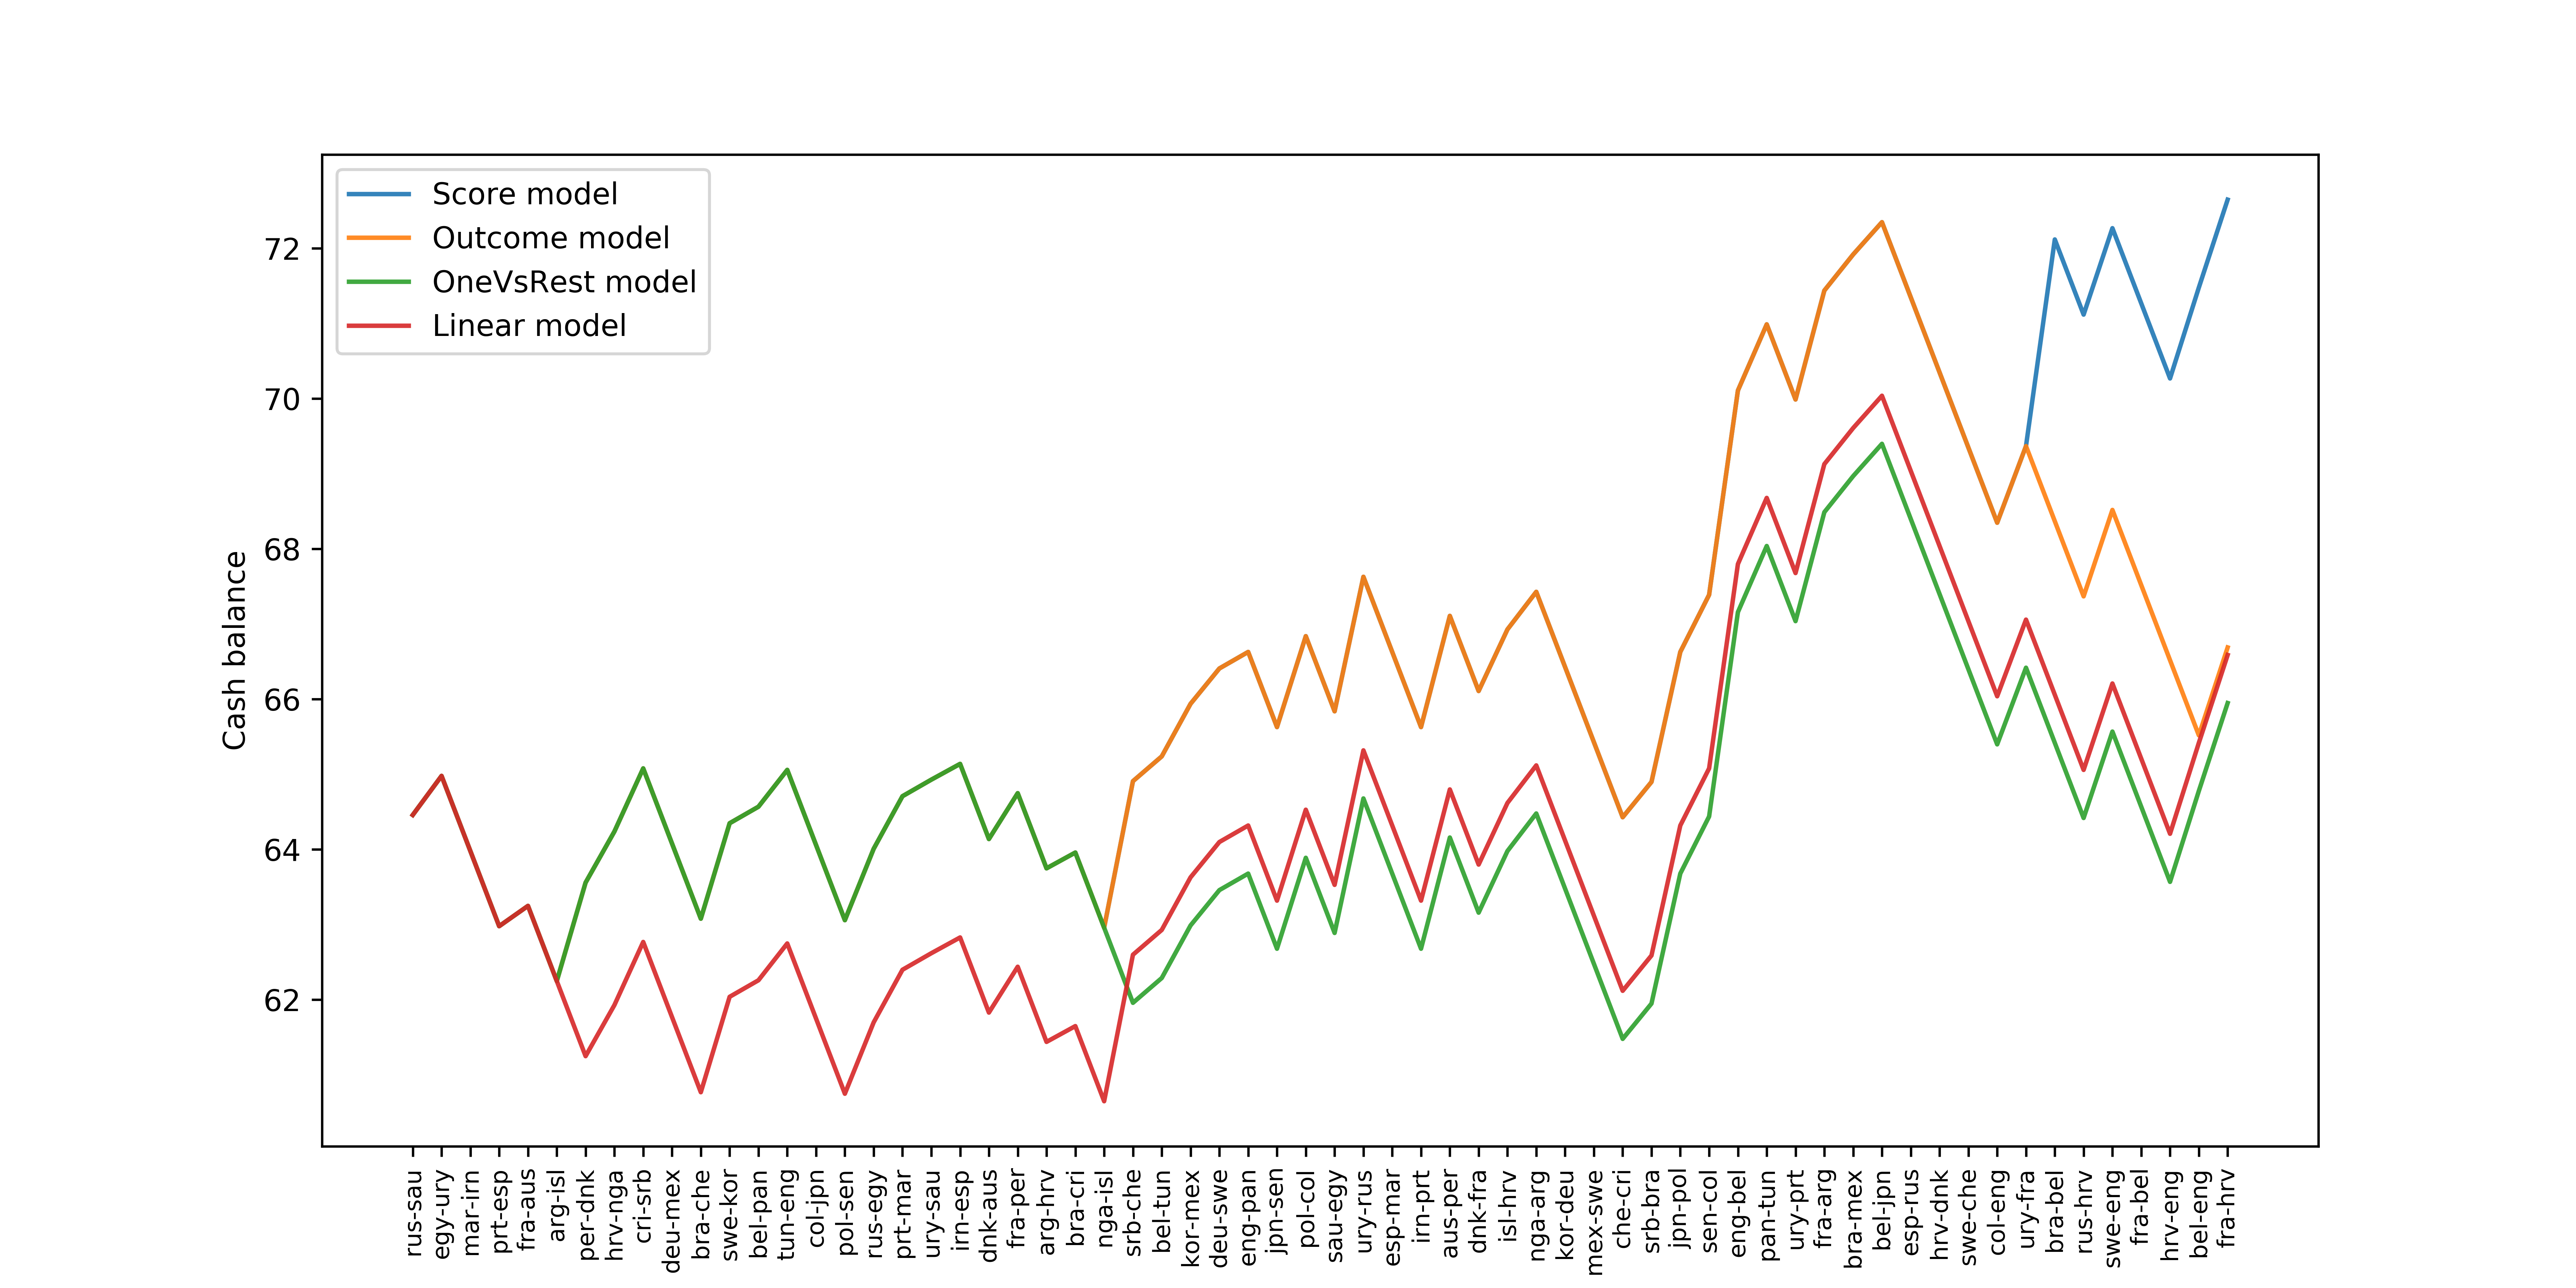
\includegraphics[width=0.7\textwidth]{img/match_level_2018_model_unit.png}
    \caption{Unit strategy's cash balance progression on World Cup 2018.}
    \label{fig:unit_model_comparison}
\end{figure}

\begin{figure}[H]
    \centering
    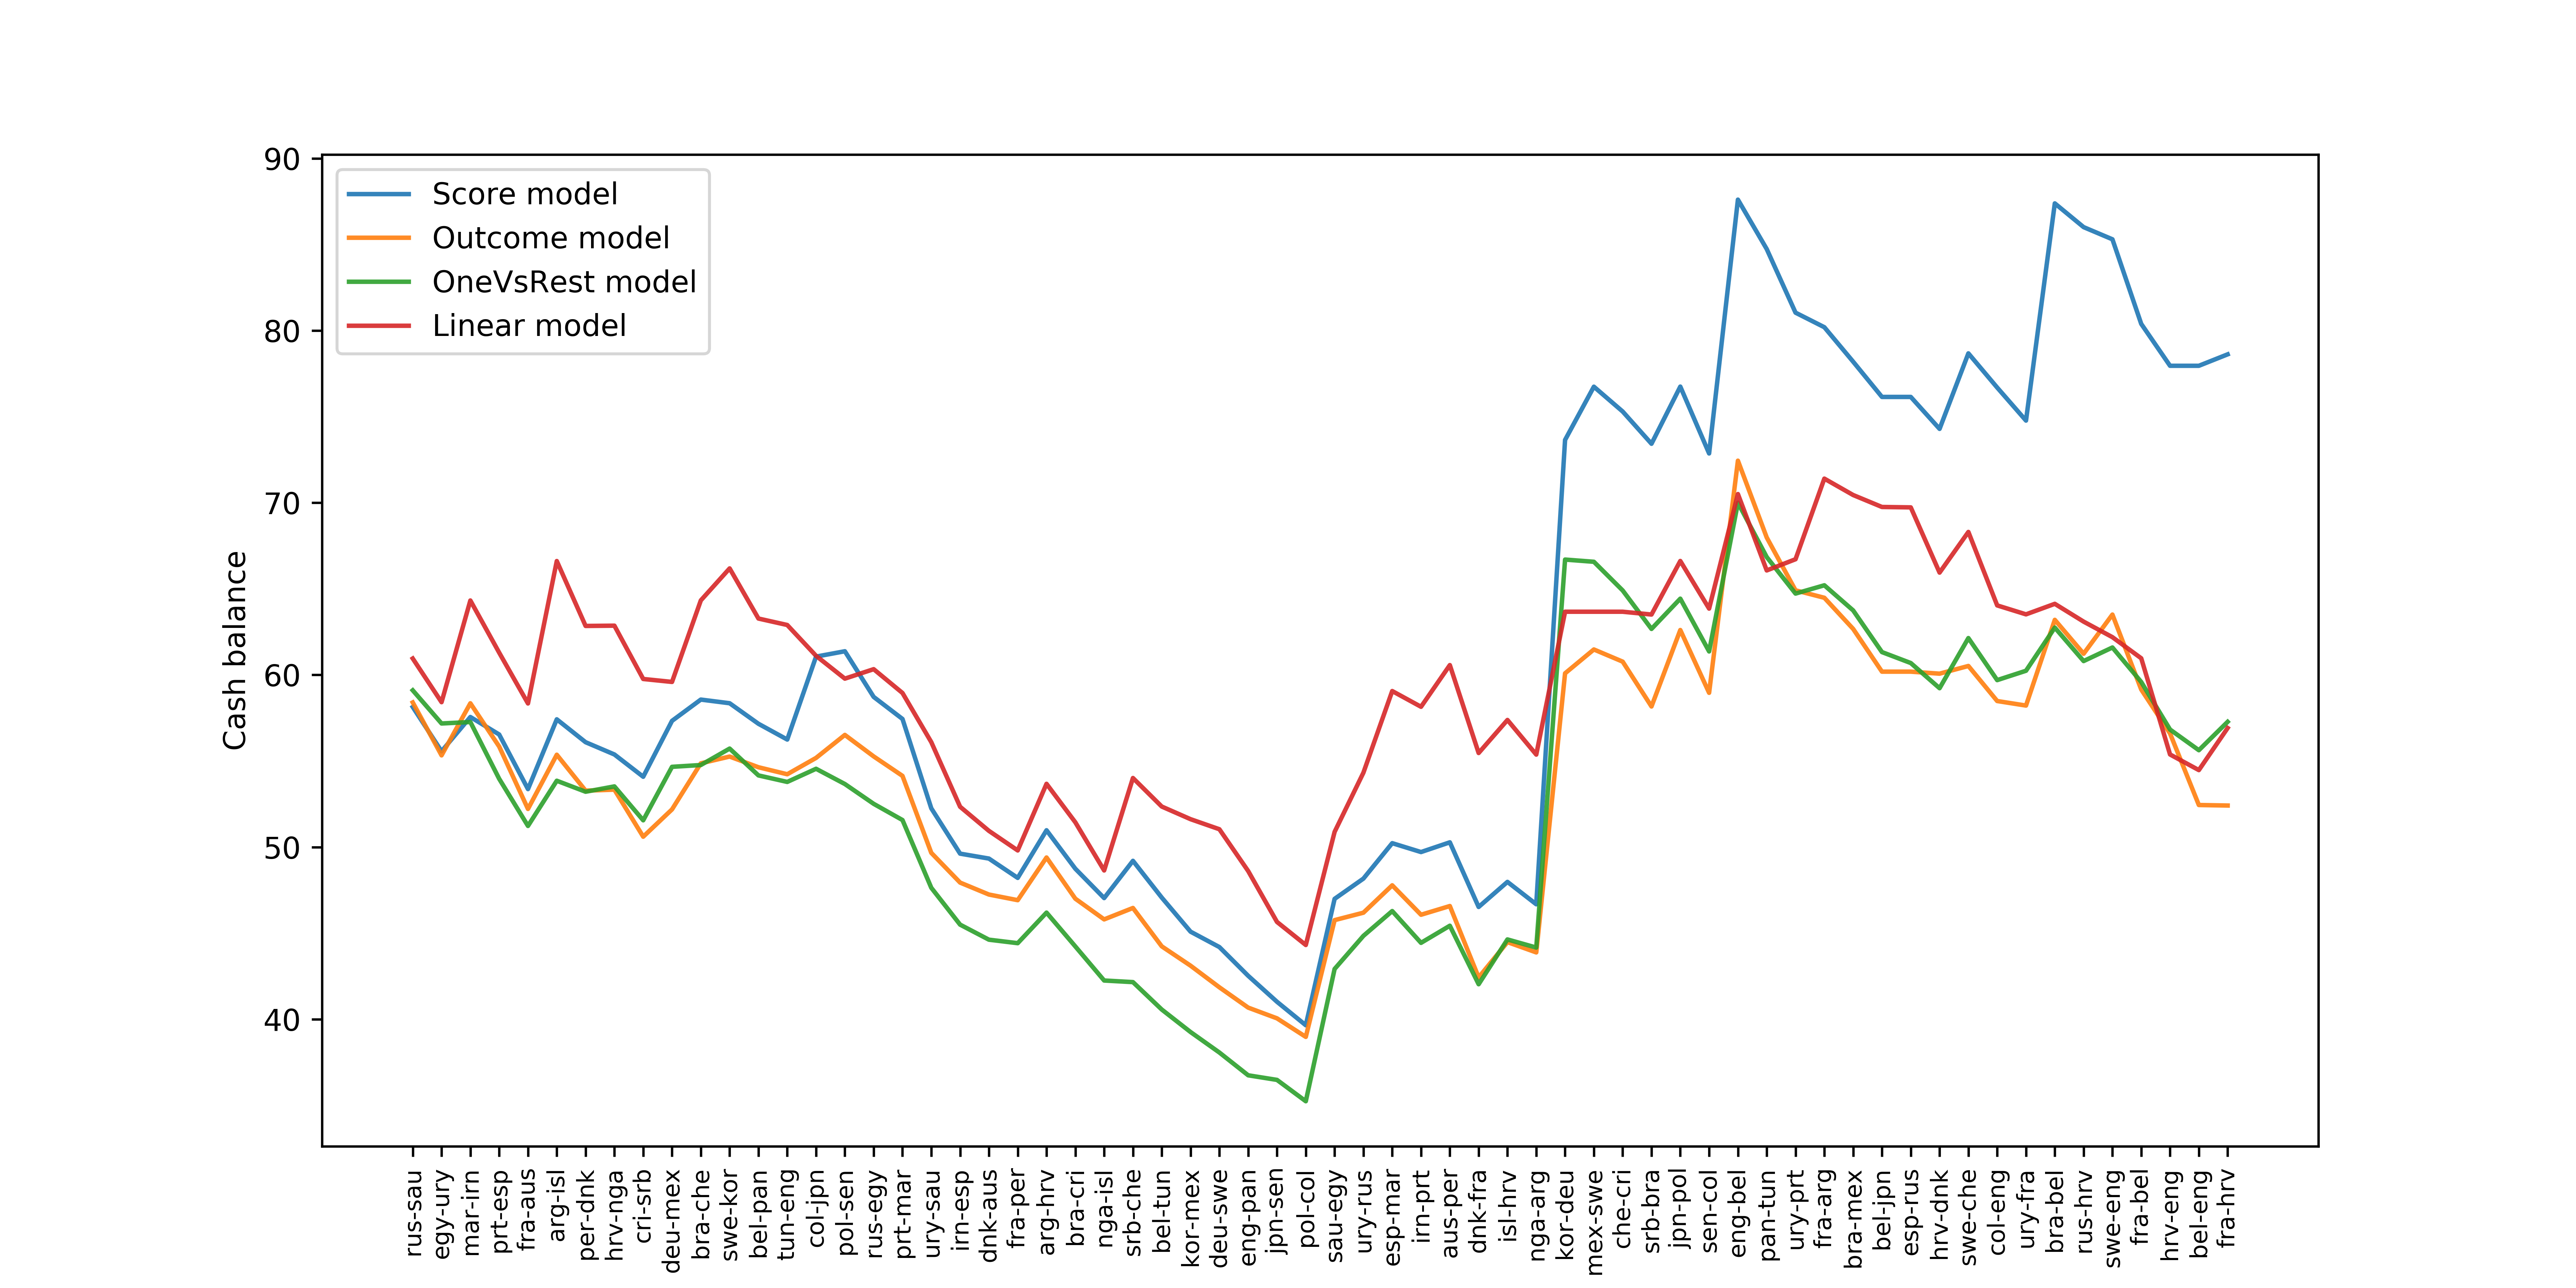
\includegraphics[width=0.7\textwidth]{img/match_level_2018_model_kelly.png}
    \caption{Kelly strategy's cash balance progression on World Cup 2018.}
    \label{fig:kelly_model_comparison}
\end{figure}

\begin{figure}[H]
    \centering
    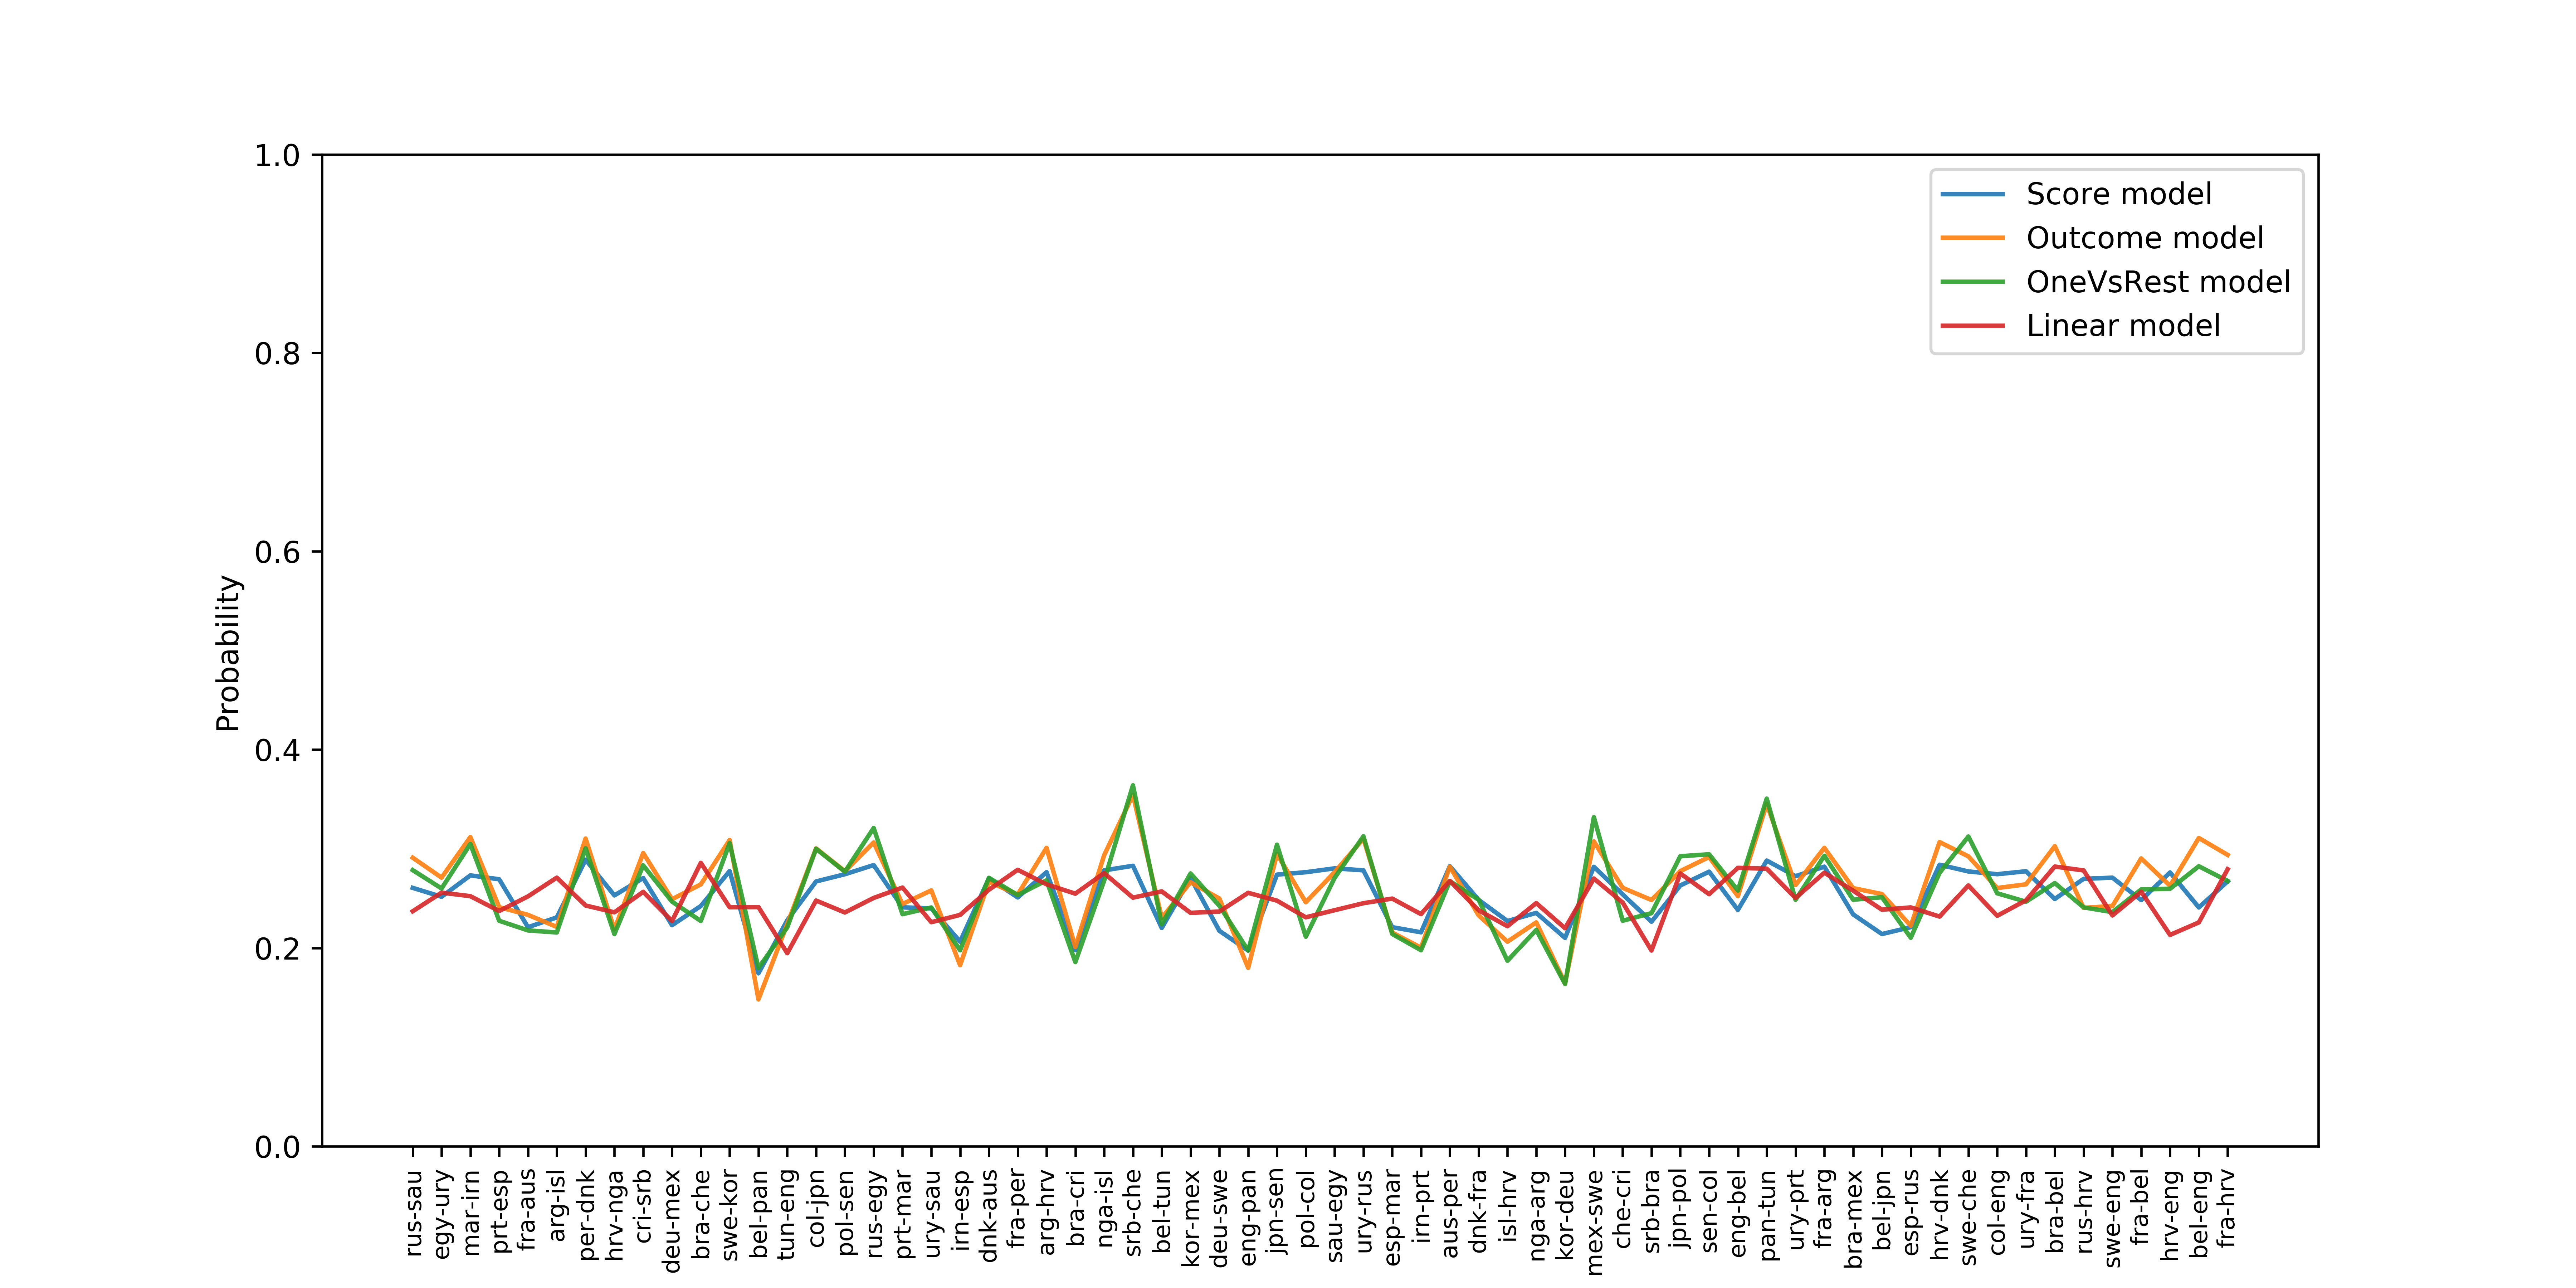
\includegraphics[width=0.7\textwidth]{img/match_level_2018_model_probability_draw_prob.png}
    \caption{Predicted probability of draw in the World Cup 2018.}
    \label{fig:draw_probability}
\end{figure}


\section{}
\subsection{Match-level betting activity}
\subsection{Feature elimination}
\subsection{Probability distribution comparison}



\begin{figure}[H]
    \centering
    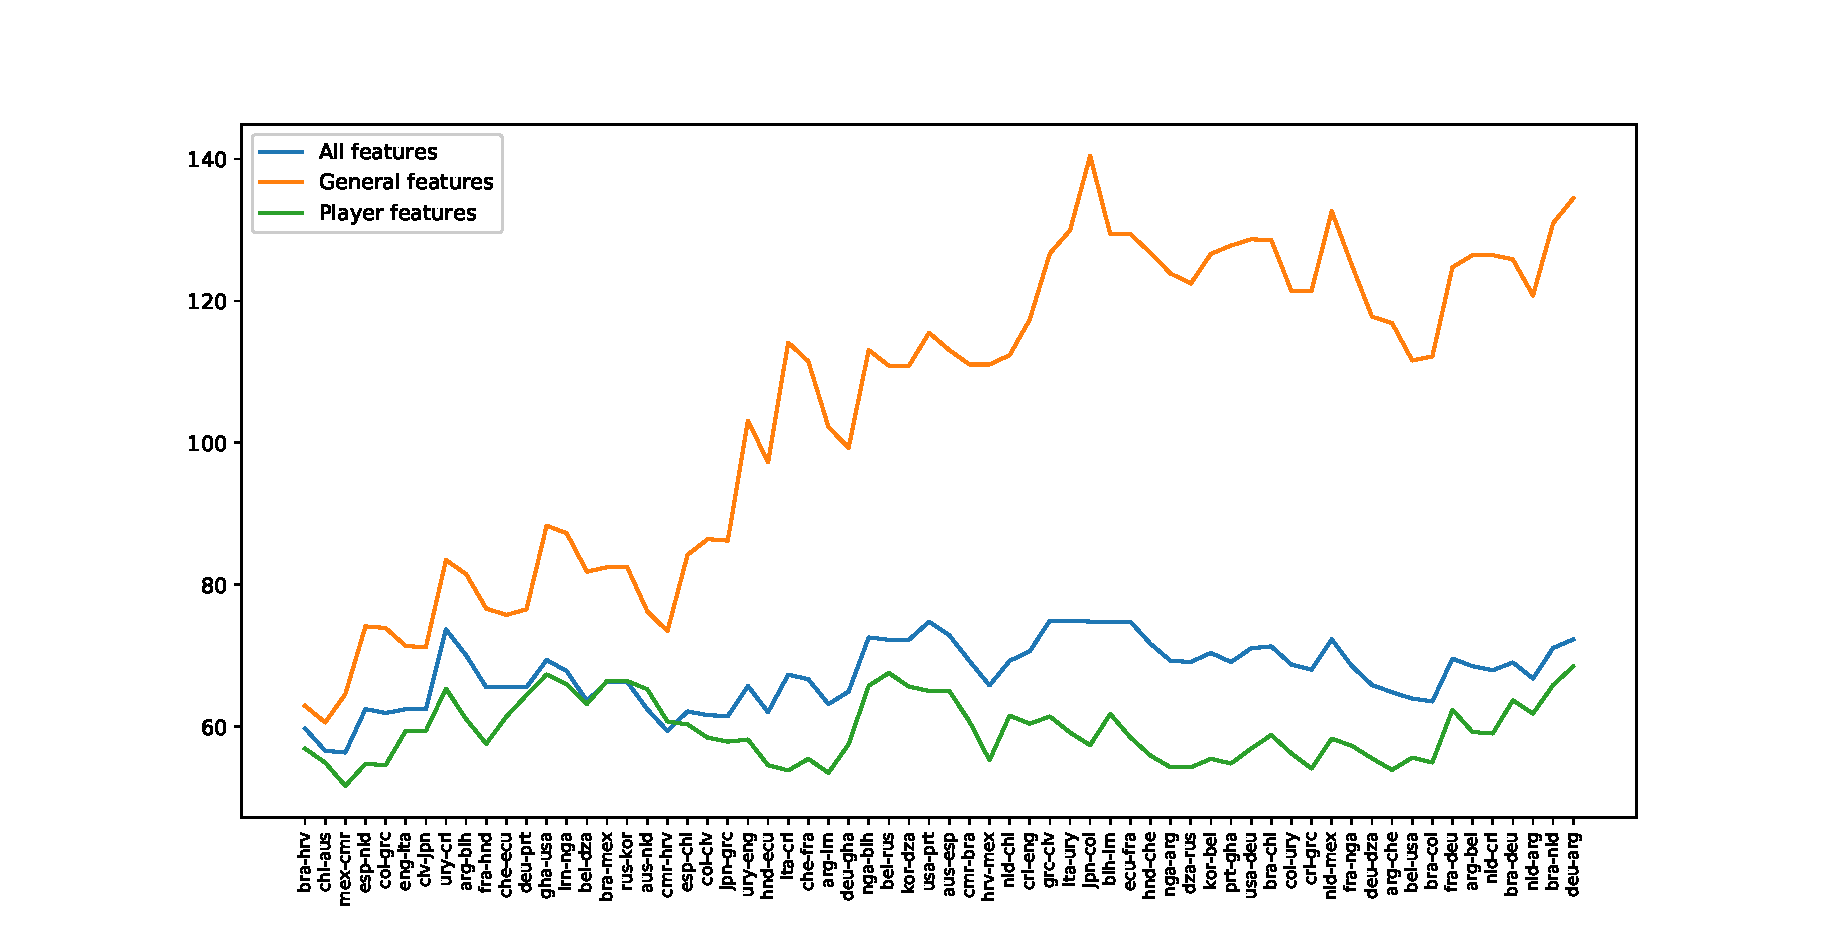
\includegraphics[width=0.7\textwidth]{img/match_level_score_2014_kelly.eps}
    \caption{50\% and 95\% tolerance ellipses.}
    \label{fig:50_95}
\end{figure}